\draft Classic optical properties question.

\begin{parts}
	\part From Drude, we know:
	\begin{align*}
		\deri{p}{t} &= f - \frac{p}{\tau} \\
		m^* \ddot{x} + \gamma m^* \dot{x} &= qE \mathrm{e}^{i\omega t}
	\end{align*}
	
	Substitute trial solution $x(t) = x_0 \mathrm{e}^{i\omega t}$:
	\begin{gather*}
		-\omega^2 m^* x_0 + i\omega\gamma m^* x_0 = qE \\
		x_0 = \frac{qE}{\rbracket{\omega^2 - i\omega\gamma}m^*}
	\end{gather*}
	
	With the polarisation $P = Nqx$, we then have the displacement field $D$ as:
	\begin{align*}
		\Rightarrow D &= \permittivity E + P + P_\textnormal{bg} = \permittivity \epsilon_r E \mtext{with $P_\textnormal{bg}$ the background polarisation} \\
		\Rightarrow \epsilon_r &= 1 + \frac{P}{\permittivity E} + \chi_\textnormal{bg} \\
		&= 1 + \frac{Nq}{\permittivity E} \rbracket{\frac{qE}{\rbracket{\omega^2 - i\omega\gamma}m^*}} + \chi_\textnormal{bg} \\
		&= 1 + \frac{Nq^2}{m^* \permittivity} \rbracket{\frac{1}{\omega^2 - i\omega\gamma}} + \chi_\textnormal{bg} \\
		&= 1 + \frac{Nq^2}{\permittivity m^*} \rbracket{\frac{\omega^2 + i\omega\gamma}{\omega^4 + \omega^2 \gamma^2}} + \chi_\textnormal{bg}
	\end{align*}
	
	For $\omega \gg \gamma$,
	\begin{equation*}
		\epsilon_r \simeq \underbracket{1 + \chi_\textnormal{bg}}_{\epsilon_\infty} + \underbracket{\frac{Nq^2}{\permittivity m^*}}_{\omega_p^2 \epsilon_\infty} \rbracket{\frac{1}{\omega^2} + i\frac{\gamma}{\omega^3}}
	\end{equation*}
	
	So $\epsilon_r = \epsilon^\prime + i \epsilon^{\prime\prime}$ where:
	\begin{align*}
		\epsilon^\prime &\simeq \epsilon_\infty - \frac{\omega_p^2}{\omega^2} \epsilon_\infty = \epsilon_\infty \rbracket{1 - \frac{\omega_p^2}{\omega^2}} \\
		\epsilon^{\prime\prime} &\simeq \epsilon_\infty \omega_p^2 \rbracket{\frac{\gamma}{\omega^3}} = \epsilon_\infty \rbracket{\frac{\gamma \omega_p^2}{\omega^3}} \mtext{with $\omega_p^2 = \dfrac{Nq^2}{\epsilon_\infty \permittivity m^*}$}
	\end{align*}
	
	\part Reflectivity $R = \abs{\dfrac{\tilde{n} - 1}{\tilde{n} + 1}}^2$ where $\tilde{n} = \sqrt{\epsilon_r}$:
	\begin{align}
		\Rightarrow R &= 0 \mtext{when $\tilde{n} = 1$} \notag \\
		\Rightarrow \epsilon_r &= 1 \notag \\
		\epsilon^\prime &\simeq 1 \mtext{since we assume $\epsilon^\prime \gg \epsilon^{\prime\prime}$} \notag \\
		\Rightarrow \epsilon_\infty \rbracket{1 - \frac{\omega_p^2}{\omega^2}} &= 1 \notag \\
		\frac{\omega_p^2}{\omega^2} &= 1 - \frac{1}{\epsilon_\infty} \label{eqn:q5-omega-condition}
	\end{align}
	
	Wavelength $\lambda = \dfrac{2\pi}{k}$ and $\dfrac{\omega}{k} = cn = c$ since $\epsilon_r = 1 \Rightarrow n = 1$:
	\begin{equation}
		\Rightarrow \lambda = \frac{2\pi c}{\omega}
		\label{eqn:q5-lambda-condition}
	\end{equation}
	
	Combining \eqref{eqn:q5-omega-condition} and \eqref{eqn:q5-lambda-condition} gives:
	\begin{align*}
		\lambda_\textnormal{min} &= 2\pi c \cdot \sbracket{\frac{1}{\omega_p^2} \rbracket{1 - \frac{1}{\epsilon_\infty}}}^{1/2} \\
		&= 2\pi c \omega_p^{-1} \rbracket{1 - \epsilon_\infty^{-1}}^{1/2}
	\end{align*}
	
	We estimate $\lambda_\textnormal{min}$ from the given graph:
	\begin{equation*}
		\lambda_\textnormal{min} = \begin{cases}
			\SI{23.5}{\micro\metre} \qquad \textnormal{(A)} \\
			\SI{20}{\micro\metre} \qquad \textnormal{(B)} \\
			\SI{15}{\micro\metre} \qquad \textnormal{(C)} \\
			\SI{9.5}{\micro\metre} \qquad \textnormal{(D)}
		\end{cases}
	\end{equation*}
	
	Thus:
	\begin{align*}
		\lambda_\textnormal{min}^2 &= \rbracket{2\pi c}^2 \rbracket{1 - \epsilon_\infty^{-1}} \cdot \frac{\epsilon_\infty \permittivity m^*}{Nq^2} \\
		\Rightarrow m^* &= \rbracket{\frac{\rbracket{2\pi c}^2 \rbracket{\epsilon_\infty - 1} \permittivity}{Nq^2 \lambda_\textnormal{min}^2}}^{-1}
	\end{align*}
	
	From the graph we estimate $R(\omega\rightarrow\infty) = \dfrac{1}{2}$:
	\begin{align*}
		\Rightarrow \abs{\frac{\sqrt{\epsilon_\infty} - 1}{\sqrt{\epsilon_\infty} + 1}}^2 &= \frac{1}{2} \\
		\sqrt{\epsilon_\infty} - 1 &= \sqrt{\frac{1}{2}} \sqrt{\epsilon_\infty} + \sqrt{\frac{1}{2}} \\
		\sqrt{\epsilon_\infty} &= \frac{1 + \sqrt{\diagfrac{1}{2}}}{1 - \sqrt{\diagfrac{1}{2}}} \\
		\epsilon_\infty &= \rbracket{\frac{1 + \sqrt{\diagfrac{1}{2}}}{1 - \sqrt{\diagfrac{1}{2}}}}^2 = \num{34.0}
	\end{align*}
	
	So we have:
	\begin{align*}
		m_\textnormal{A}^* &= \num{0.05}m_e \\
		m_\textnormal{B}^* &= \num{0.06}m_e \\
		m_\textnormal{C}^* &= \num{0.09}m_e \\
		m_\textnormal{D}^* &= \num{0.12}m_e
	\end{align*}
	Note that the effective mass increases as $N$ increases, this is due to the fact that the valence band is populated with more holes, thereby lowering the chemical potential and render $m^*$ greater:
	\begin{figure}[H]
		\centering
		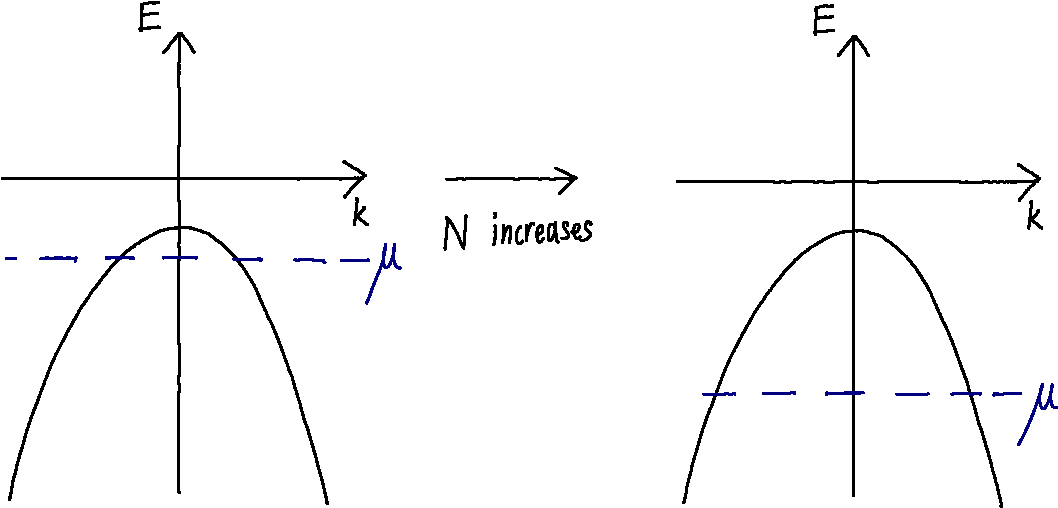
\includegraphics[width=.8\linewidth]{q5-density-chempot}
	\end{figure}
	
	\part Mobility $\mu = \dfrac{e\tau}{m^*}$.
	
	We observe that $\lambda_\textnormal{min}$ increases as $T$ increases, thereby suggesting $m^*$ decreases from before.
	
	Lower $m^*$ thus increases $\mu$ for a constant $\tau$.
	
	However we know $\tau$ decreases due to larger thermal agitation so we expect $\mu$ to decrease at large $T$.
\end{parts}